%%%%%%%%%%%%%%%%%%%%%%%%%%%%%%%%%%%%%%%%%%%%%%%%%%%%%%%%%%%%%%%%%%%%%%%%%%%%%
%
%  System        : 
%  Module        : 
%  Object Name   : $RCSfile$
%  Revision      : $Revision$
%  Date          : $Date$
%  Author        : $Author$
%  Created By    : Robert Heller
%  Created       : Sat Apr 15 10:33:56 2023
%  Last Modified : <230415.1033>
%
%  Description 
%
%  Notes
%
%  History
% 
%%%%%%%%%%%%%%%%%%%%%%%%%%%%%%%%%%%%%%%%%%%%%%%%%%%%%%%%%%%%%%%%%%%%%%%%%%%%%
%
%    Copyright (C) 2023  Robert Heller D/B/A Deepwoods Software
%			51 Locke Hill Road
%			Wendell, MA 01379-9728
%
%    This program is free software; you can redistribute it and/or modify
%    it under the terms of the GNU General Public License as published by
%    the Free Software Foundation; either version 2 of the License, or
%    (at your option) any later version.
%
%    This program is distributed in the hope that it will be useful,
%    but WITHOUT ANY WARRANTY; without even the implied warranty of
%    MERCHANTABILITY or FITNESS FOR A PARTICULAR PURPOSE.  See the
%    GNU General Public License for more details.
%
%    You should have received a copy of the GNU General Public License
%    along with this program; if not, write to the Free Software
%    Foundation, Inc., 675 Mass Ave, Cambridge, MA 02139, USA.
%
% 
%
%%%%%%%%%%%%%%%%%%%%%%%%%%%%%%%%%%%%%%%%%%%%%%%%%%%%%%%%%%%%%%%%%%%%%%%%%%%%%

\subsection{Siding with local control panel}
\label{sect-appl:siding}
\begin{figure}[hbpt]\begin{centering}%
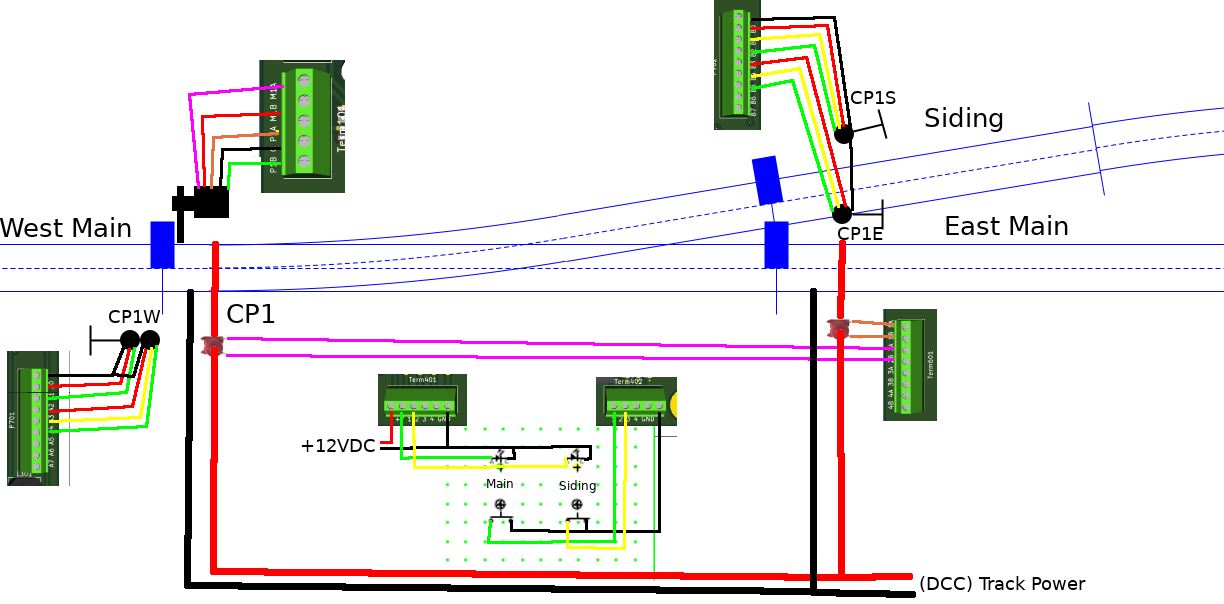
\includegraphics[width=5in]{ExampleSidingCP1-Wiring.png}
\caption{One end of a siding (CP1) with local and remote control, with 
signals.}
\label{fig:ExampleSidingCP1-Wiring}
\end{centering}\end{figure}

This is a basic single turnout with a facia panel with two LEDs indicating the
turnout points' position and two push buttons to select the desired turnout
position. There also is a two headed (3 over 2) interlocking signal at the
turnout's points, and a pair of single head (3 color) signals at the frog
ends. The turnout's wiring is shown in 
Figure~\ref{fig:ExampleSidingCP1-Wiring}. We will use one of the turnout 
drivers (the Stall Motor daughter board is shown, but any of the daughter 
boards could be used), two of the occupancy detectors, two of the LED drivers, 
two of button inputs, and 11 of signal lamp driver outputs.

We will start by configuring the user name and description of the node in User 
Info tab.  When we have done this will will be able to find the node by 
looking for the name.  

Next, we will move onto the Board Configuration tab and then the Occupancy
Detectors, specificly OC1. Right now, we will just fill in the name (East
Main) and create a Block layout control. Similarly for OC2 (CP1 OS).

Similarly we configure the Turnout and Points, filling their names and
creating layout control elements for them, along with the veto control
element. The layout coltrol elements (or various JMRI table elements). 

Next we set up the logic for the Veto. We want to enable the turnout veto in
two cases: dispatcher locking or OS occupancy, so we need one logic element
for this. We name the Logic ``Veto On'', copy the OS Occupancy detector events
to Variable 2 (Variable 1 will be used by the dispatcher to lock the turnout),
set the Logic to V1 OR V2. The actions for both true and false will be send
and exit. Action event 1 will be Send Immediately on True and the Turnout Veto
On event will be copied to the action event. Action event 2 will be Send
Immediately on False and the the Turnout Veto Off event will be copied to the
action event.

Next we set up the LED drivers and the button inputs. We copy the turnout's
Normal and Reverse motor events to the two button ON events and label the
buttons Normal and Reverse. Simularly we copy the Point sensor events to the
LEDs' events. For the Normal labeled LED, copy the Point sensor Normal event
to the on event, and the Point sensor Reverse event to the off event. Then for
the Reverse labeled LED, copy the Point sensor Reverse event to the on event, 
and the Point sensor Normal event to the off event.

For the signals, we will use additional Logics and three Masts.  For each 
signal will will construct an sequense of logic elements, one for each aspect, 
starting with the most restrictive and ending with the least restrictive.  
Each logic element will test one or two conditions and be true for one aspect.

For the signal at the point entry of the turnout we are using a two headed
signal, a 3 over 2 (3 lamps (GYR) on the top head, 2 lamps (GR or YR) on the
bottom head). This signal will display 4 aspects: Stop (red over red),
Approach Limited (red over green or yellow), Approach (yellow over red), and 
Clear (green over red).  These aspects mean: 

\begin{itemize}
\item Stop (red over red) Absolute stop.  Typically because the turnout is 
currently occupied or the dispatcher forbids traversal.
\item Approach Limited (red over green or yellow) Slow speed, taking the 
siding.  This is when the turnout is thrown.
\item Approach (yellow over red) Reduced speed continuing on the main.  This 
is when there is a Stop indication at the next signal.
\item  Clear (green over red) Normal speed continuing on the main.  This is 
when no other cases prevail.
\end{itemize}

Select the Mast 1 tab under the Rule to aspect tab under Board Configuration. 
Select Normal under Mast Processing and enter a Mast ID of CP1W for the Mast 
ID.  Then copy the Track Circuit Link Address to Circuit 1 under TRACK 
CIRCUITS and set the Remote Mast Description  to CP1W.

Back at Rule to aspect / Mast 1 scroll down to the Rules. Under Rule 1's
Appearance, set Lamp 1 to A0, and Lamp 2 to A2. These are the two red lamps.
Now select tab Rule 2.  Set Name to 27-Approach-Limited and Track Speed to 
Limited.  Then for its Appearance, set Lamp 1 to A1 and Lamp 2 to A2. Moving 
on to Rule 3: Set Name to 21-Approach and Track Speed to Approach.  Then Lamp 
1 to A0, and Lamp 2 A3.  Finally for Rule 4: Set Name to 29-Clear and Track 
Speed to Clear/Procede and Lamp 1 to A0, and Lamp 2 to A4. This completes 
setting up the mast.

The logic for this mast is:

\begin{verbatim}
if (TurnoutOS is occupied) then
    send Stop
else if (Turnout is Reversed) then
    send Approach Limited
else if (track circuit(next block) is Stop) then
    send Approach
else
    send Clear
\end{verbatim}

We will need 4 successive Logic elements for this mast, but first we need to 
create a virtual mast for the block identified as East Main.  We will use Mast 
8 and Circuit 8 for this mast.  Select Mast 8, set its Mast Processing to 
Normal, its Mast ID to CP1ME, and copy its Link Address to Circuit 8.  Now 
right click on the East Main OC in the Layout DB window, and copy its Occupied 
event to the event to set aspect for Rule 1 (Rule one is already set to Stop 
speed).  Then copy East Main's Clear event to the event to set aspect for Rule 
2, then change Rule 2's name to 29-Clear and Track Speed tp Clear/Procede.  We 
won't be setting anything for this mast's Lamps, since it is not a ``visible'' 
signal.  We are just using it to general track circuit signals.

Now we can start to set up the Logic elements. We will start with Logic 4. Set
its description to ``CP1W Stop'', its Group Function to Group, copy CP1 OS OC
detector's events to Variable \#1's events: true from Occupied, false from
Clear. Set the Logic function to V1 only, set Action 1 to Immediate If True
and copy the event from Mast 1, Rule 1's ``(C) Event to Set Aspect'' event to 
Action 1's event.

Next we set up Logic 5. Set its description to ``CP1W Approach Limited'', its 
Group Function to Group, copy the Points 1 sense detector's events to Variable 
\#1's events: true from Reversed, false from Normal -- we want *true* if the 
turnout is set to the siding. Set the Logic function to V1 only, set Action 1 
to Immediate If True  and copy the event from Mast 1, Rule 2's ``(C) Event to 
Set Aspect'' event to Action 1's event.

Next we set up Logic 6. Set its description to ``CP1W Approach'', its Group 
Function to Group, its variable source to Track Circuit 8.  Use the default 
speed of Stop.  Set the Logic function to V1 only, set Action 1 to Immediate 
If True  and copy the event from Mast 1, Rule 3's ``(C) Event to Set Aspect'' 
event to Action 1's event.

Finally we set up Logic 7. Set its description to ``CP1W Clear'', its Group 
Function to Last (Single), set its Logic function to null $=>$ true, set Action 
1 to Immediate If True  and copy the event from Mast 1, Rule 4's ``(C) Event 
to Set Aspect'' event to Action 1's event.

Next we need to set up the two signals at the frog end of the turnout.  They 
both the same aspects:

\begin{itemize}
\item Stop (red) Absolute stop.  Typically because the turnout is currently 
occupied, the points are aligned against travel, or the dispatcher forbids 
traversal.
\item Approach (yellow) Reduced speed continuing on the main.  This is when 
there is a Stop indication at the next signal.
\item  Clear (green) Normal speed continuing on the main.  This is when no 
other cases prevail.
\end{itemize}

We will set up these two signals on Mast 2 and Mast 3 and also set up a 
virtual mast for West Main using Mast 7.

First CP1E on Mast 2:

Set Mast Processing to Normal, Mast ID to CP1E, copy the track circuit address 
to Circuit 2, along with the Mast ID to the Remote Mast Description. Rule 1's
Name will be 0-Stop, its speed Stop, and its Appearence will be Lamp 1: B3.
Rule 2's Name will be 21-Approach, its speed Approach, and its Appearence will 
be Lamp 1: B4. Rule 3's Name will be 29-Clear, its speed Clear/Procede, and 
its Appearence will be Lamp 1: B5.

Then CP1S on Mast 3:

Set Mast Processing to Normal, Mast ID to CP1S, copy the track circuit address 
to Circuit 3, along with the Mast ID to the Remote Mast Description. Rule 1's
Name will be 0-Stop, its speed Stop, and its Appearence will be Lamp 1: B0.
Rule 2's Name will be 21-Approach, its speed Approach, and its Appearence will 
be Lamp 1: B1. Rule 3's Name will be 29-Clear, its speed Clear/Procede, and 
its Appearence will be Lamp 1: B2.






\clearpage
